\documentclass{report}
\usepackage[margin=1in]{geometry}
\usepackage{setspace}
\usepackage{times}
\usepackage{pdfpages}
\title{
	\textsc{ \small
		Washington State University \\
		School of Electrical Engineering and Computer Science \\
		EE 352, Electrical Engineering Laboratory
	} \\
	{\textsc{\small Lab \#3}} \\
	Operational Amplifier Applications
}

\author{
	Name: Kevin Evans \\
	Partner: Jacob Hnatiak
}
\date{Due Date: February 11, 2020}


% start sections at 1 with subsections to 1.1, 1.2...
\renewcommand{\thesection}{\arabic{section}}

%alias for vpp/rms
\newcommand{\pp}{_{pp}}
\newcommand{\rms}{_{rms}}
\newcommand{\Vpp}{\V\pp}
\newcommand{\Vrms}{\V\rms}

\usepackage{pgfplots}
\usepackage{filecontents}

\usepackage{clipboard}
\usepackage{siunitx}
\usepackage{threeparttable}
\usepackage{booktabs}
\usepackage{multirow}
\usepackage{graphicx}
\usepackage{float}
\usepackage{amssymb,amsmath}
\usepackage{physics,cancel}

\usepackage{steinmetz} % \phase{}
\usepackage{mathtools} % for '\mathclap' macro
\usepackage{caption,subcaption} %multiline captions; subfigures

\sisetup{inter-unit-product=\cdot}
%\usepackage{filecontents}
%\begin{filecontents*}[overwrite]{general.bib}
%	@manual{ad:op27,
%		organization  = "Analog Devices",
%		title         = "Low Noise, Precision Operational Amplifier",
%		number        = "OP27",
%		year          =  2006,
%		month         =  5,    
%		note          = "Rev. F"
%	}
%\end{filecontents*}

\usepgfplotslibrary{units}

%\usepackage{biblatex}
%
%\addbibresource{general.bib}
%\nocite{*}

\begin{document}
	\maketitle
	
	\section*{Lab Overview}
	% what was the lab about and the outcome?
	The lab demonstrated several use-cases of operational amplifiers. The first experiment used the OP27 op amp to double the voltage of high frequencies and attenuate low frequencies. Next, cascading amplifiers were used in a design featuring a high gain output, with low output resistance and a high input resistance.
	
	\section{First Order High Pass Active Filter}
	
	\subsection{Purpose}
	% purpose of the experiment and its specs and/or design requirements
	The purpose of this experiment was to implement an active high-pass filter using an OP-27 op-amp and an RC circuit. The circuit would be used to amplify high frequency signals to \SI{6}{\dB} and attenuate low frequency signals. 
	
	
	\subsection{Theoretical background}
	% background and its theory of operation, circuit diagrams, the main equations, results from the prelab
	
	Op amps are often used in filtering applications, and has several advantages over passive filters. In this experiment, we will construct an active filter using the OP-27 amplifier. The filter will be a high-pass type and is shown below in Figure \ref{fig:exp1filter}. 
	
	\begin{figure}[h]
		\centering
		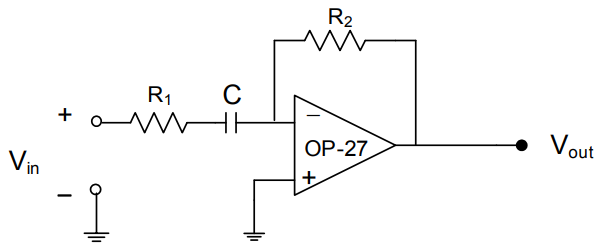
\includegraphics[width=0.5\linewidth]{exp1filter}
		\caption{The active filter circuit used in this experiment.}
		\label{fig:exp1filter}
	\end{figure}

	\subsubsection{Time domain}
	In the time domain, we can characterize this circuit using a differential equation. If we assume an ideal op amp and perform KCL along the top current, we can say that the input current across the capacitor is equal to the feedback current, across $R_2$. The relationship between $V_\mathrm{out}$ and $V_\mathrm{in}$ becomes,
	\begin{equation}
		\dv{V_\mathrm{out}}{t} + \frac{1}{R_1 C} V_\mathrm{out} = -\frac{R_2}{R_1} \dv{V_\mathrm{in}}{t} \label{eq:exp1diffeq}
	\end{equation}
	The solution to \eqref{eq:exp1diffeq} are a real or complex exponential, depending on the input voltage. For a real exponential, where the input voltage is constant, such as with a step response, the function will have a time constant $\tau$ of
	\begin{equation}
		\tau = R_1 C \label{eq:exp1tau}
	\end{equation}

	\subsubsection{Phasor domain}
	Using phasors, we can treat each element with their corresponding impedances and determine the amplitude response. This greatly simplifies the analysis. The input and feedback impedance become
	\begin{subequations}
		\begin{align}
			Z_\mathrm{in} & = R_1 + \frac{1}{j\omega C} \\
			Z_\mathrm{fb} & = R_2
		\end{align}
	\end{subequations}
	If we again assume an ideal op amp with zero input current, we can simply use KCL and KVL, then would find the amplifier's gain,
	\begin{align}
	\frac{V_\mathrm{out}}{V_\mathrm{in}} & = -\frac{R_2}{R_1 + \frac{1}{j\omega C}} \label{eq:exp1gain}
	\end{align}
	For the amplitude only, we can take the magnitude of the gain,
	\begin{align}
		\frac{\abs{V_\mathrm{out}}}{\abs{V_\mathrm{in}}} & = \frac{\omega R_2 C}{\sqrt{1 + \omega^2 R_1^2 C^2}} \label{eq:exp1dcgain}
		%
		%& = K 
	\end{align}
	If we take the limits of the frequency, at $\omega = 0$, the low frequency (DC) gain is zero. At higher frequencies, $\omega \to \infty$, the gain is proportional to $R_2 / R_1$. This indicates that the circuit is correctly acting as a high-pass filter with an additional gain.
	
	\subsubsection{Cutoff frequency}
	The cutoff frequency can be determined using both the time and phasor domain. From the time domain, the cutoff frequency is given by the inverse of \eqref{eq:exp1tau}. In the phasor domain, we can determine the cutoff frequency using \eqref{eq:exp1gain}. From inspection, we can see the denominator of the gain must equal $\sqrt{2}$, \begin{align}
		\frac{\abs{V_\mathrm{out}}}{\abs{V_\mathrm{in}}} & = \frac{1}{\sqrt{2}}  \notag \\
		1 + \omega_0^2 R_1^2 C^2 & = 2 \notag \\
		\omega_0 & = \frac{1}{R_1 C} \label{eq:exp1cutoff}
	\end{align}

	
	\subsubsection{Amplifier design}
	The amplifier design had three requirements: (1) an input resistance of $R_1 = \SI{10}{\kohm}$, (2) a high frequency gain of \SI{6}{\dB}, and lastly (3) a cutoff frequency of \SI{300}{\Hz}. In order to meet these requirements, the values of $C$ and $R_2$ must be chosen accordingly. For a cutoff frequency of \SI{300}{\Hz}, we can use \eqref{eq:exp1cutoff} to determine the required capacitance
	\begin{align*}
		\omega_0 & = \frac{1}{R_1 C} = 2 \pi \left( \SI{300}{\Hz}\right) \\
		C & = \frac{1}{2 \pi \left(\SI{10}{\kohm}\right)\left(\SI{300}{\per \second}\right)} \\
			& = \SI{53.1}{\nano\farad}
	\end{align*}
	The value of $R_1$ can be determined from the \SI{6}{\dB} requirement and by taking the high frequency limit of \eqref{eq:exp1dcgain}, \begin{align*}
		\SI{6}{\dB} & = \SI{2}{\V/\V} = R_2 / R_1\\
		R_1 & = 2 \left( \SI{10}{\kohm}\right) \\
			& = \SI{20}{\kohm}
	\end{align*}
	With these values, the circuit can easily be simulated in PSPICE and the requirements can be verified, shown by the Bode plot in Figure \ref{fig:exp1simscreenshot} (Appendix).
	
	\pagebreak
	
	\subsection{Procedure}
	The follow steps were carried out, as instructed by the lab assignment.
	\begin{enumerate}
		\item The circuit shown in Figure \ref{fig:exp1filter} was constructed.
			\begin{enumerate}
				\item The IC pinout, shown in Figure \ref{fig:exp1pinout} (Appendix), from the OP27 datasheet was used.
				\item The Rigol DP832 was used to create a \SI{+12}{\V}, \SI{-12}{\V}, and \SI{0}{\V} ground supply for the OP-27.
				\item The \SI{+12}{\V} and \SI{-12}{\V} was attached to pin 7 and 4 of the OP-27 respectively.
				\item The input signal $V_{in}$ was generated by the function generator and attached to pin 2.
				\item The circuit was verified correct by the TA.
			\end{enumerate}
		
		\item To experimentally see the step response, a \SI{1}{\Vpp} square wave was generated with a \SI{0.5}{\V} offset and attached to $V_{in}$ of the circuit. The frequency was initially set to \SI{300}{\Hz} and was reduced to \SI{20}{\Hz} to view the response until nearly equilibrium.
		
		\item Next, the function generator was set to use \SI{4}{\Vpp} sine wave output with \SI{0}{\V} offset in order to determine the frequency response. The frequency was swept from \SI{30}{\Hz} to \SI{1}{\MHz}, with careful attention spent around the expected cutoff frequency of \SI{300}{\Hz}. These data points were recorded in Excel and plotted.
	\end{enumerate}
	
	\subsection{Results and analysis}
	% state all measured values, graphs, tables, and figs.
	% state any deviation from theoretical expected values
	% use tables and graphs
	% * must justify error in results otherwise the experiment failed
	
	\subsubsection{Measured component values}
	The measured component values are shown in Table \ref{table:lab1components}. 
	As \SI{53}{\nano\farad} capacitors were not available, we instead chose a network of capacitors, with $C_1$ in series with $C_2$, then both in parallel with $C_3$. Using the individual capacitances, one would expect the equivalent capacitance to be \SI{55.8}{\nano\farad}. However, once attached to the breadboard, the capacitance was measured to be $C_\mathrm{eq} \approx \SI{53}{\nano\farad}$. This is likely due to the stray capacitance. of the board.
	
	\begin{table}[h]
		\centering
		\caption{Experimental and nominal component values.}
		\label{table:lab1components}
		\begin{threeparttable}
			\begin{tabular}{cccc}
				\toprule
				Component & Nominal & Measured & \% Error (Tolerance) \\
				\midrule
				$R_1$ & \SI{10}{\kohm} & \SI{9.973}{\kohm} & 2.70\% (5\%) \\
				$R_2$ & \SI{20}{\kohm} & \SI{19.40}{\kohm} & 3.00\% (5\%) \\
				$C_1$ & \SI{100}{\nano\farad} & \SI{106}{\nano\farad} & 6\% (10\%) \\
				$C_2$ & \SI{100}{\nano\farad} & \SI{98}{\nano\farad} & 2\% (10\%) \\
				$C_3$ & \SI{4.7}{\nano\farad} & \SI{4.85}{\nano\farad} & 3.2\% (10\%) \\
				\midrule
				$C_\mathrm{eq}$\tnote{1} & \SI{53}{\nano\farad} & \SI{53}{\nano\farad} & 0\% (--) \\
				\bottomrule
			\end{tabular}
			\begin{tablenotes}
				\footnotesize
				\item[1] Using the RLC meter, the equivalent capacitance $C_\mathrm{eq}$ was measured to be \SI{53}{\nano\farad} on the breadboard.
			\end{tablenotes}
		\end{threeparttable}
	\end{table}

	\subsubsection{Step response}
	The square wave input was set to $f=\SI{20}{\Hz}$ and the output voltage was found to rise from \SI{-2}{\V} to \SI{0}{\V}, shown in Figure \ref{fig:exp1step_long}. Of a \SI{2}{\Vpp} response, the expected voltage at one time constant is \SI{1.260}{\V}. However, as the output wave is inverted and offset \SI{2}{\V}, the output voltage after one time constant would be \SI{-0.740}{\V}. Shown in Figure \ref{fig:exp1step_cursors}, cursors were used to determine the time from the trigger ($t=0$) to reach \SI{-0.740}{\V}, $\Delta t=\tau=\SI{536.0}{\us}$.
	
	Using the experimental component values from Table \ref{table:lab1components}, the expected time constant using \eqref{eq:exp1tau} is \SI{515.7}{\us}, or an expected corner frequency of \SI{308}{\Hz}. The measured time constant deviated by 3.9\%. This error was relatively small, but was likely caused by the non-ideal op amp and stray impedances of the breadboard and wires. 

	\begin{figure}[h]
		\centering
		\begin{subfigure}[t]{0.5\textwidth}
			\centering
			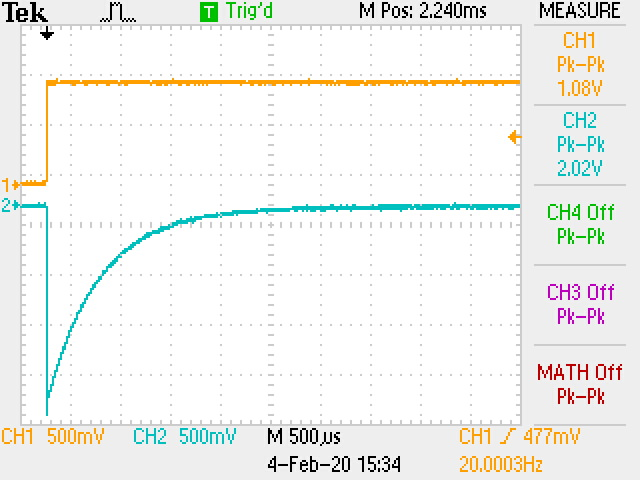
\includegraphics[width=\textwidth]{scope/F0001TEK}
			\caption{A broad (\SI{5}{\ms}) view of the step response.}
			\label{fig:exp1step_long}
		\end{subfigure}%
		~ 
		\begin{subfigure}[t]{0.5\textwidth}
			\centering
			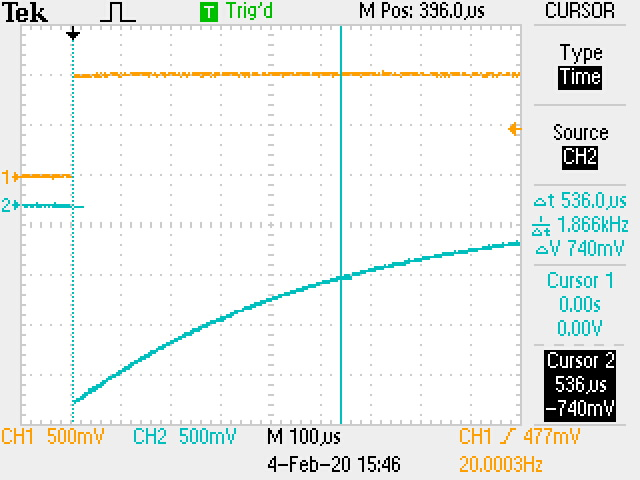
\includegraphics[width=\textwidth]{scope/F0003TEK}
			\caption{Using cursors to identify the approximate time constant $\tau$.}
			\label{fig:exp1step_cursors}
		\end{subfigure}
		\caption{Step response of the high-pass op amp circuit.}
	\end{figure}

	\subsubsection{Frequency response}
	The approximate frequency response was found by measuring the output voltage using the oscilloscope at a range of frequencies, from \SI{30}{\Hz} to \SI{1}{\MHz}. This data was plotted using Excel, shown in Figure~\ref{fig:exp1bode} below. Around the expected corner frequency of \SI{300}{\Hz}, additional points were taken to find the experimental cutoff frequency. It was found that \SI{312}{\Hz} led to a gain of \SI{2.98}{\dB}. This was 4\% from the required cutoff frequency of \SI{300}{\Hz}. This error was likely due to stray impedances of the breadboard. 
	
	Additionally, near the limits of the op amp, there is a slight uptick in the gain. It nominally should be \SI{6}{\dB}, however, it experiences nearly \SI{6.5}{\dB} near \SI{125}{\kHz}. This seems to be a second order effect, likely caused by the impedances of the breadboard or oscilloscope probes, or non-ideal characteristics of the function generator.
	
	% only 1% from the expected corner frequency using the step response.
	\begin{figure}[H]
		\centering
		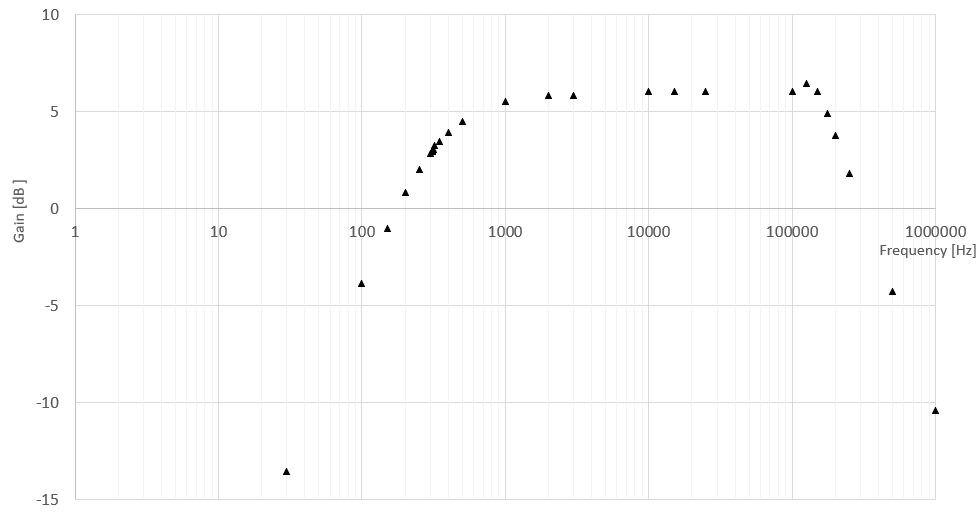
\includegraphics[width=0.75\linewidth]{exp1bode}
		\caption{Experimental frequency response of the active high-pass op amp.}
		\label{fig:exp1bode}
	\end{figure}
	
	\subsection{Conclusion}
	%  conclusion of the exp
	This experiment demonstrated an active high pass filter, enabling high frequencies to be amplified while attenuating lower frequencies. The time constant and cutoff frequency can be determined experimentally using both a step response, as well as the phasor frequency response.
	
	
	\pagebreak
	
	%%%%%%%%%%%%%%%%%%%%%%%%%%%%%%%%%%%%%%%%%%%%%%%%%%%%%%%%%%%%%%%%%%%%%%
	\section{High gain amplifier}
	
	\subsection{Purpose}
	% purpose of the experiment and its specs and/or design requirements
	This experiment involved designing a high gain amplifier using components from the previous experiment. It should have a high input resistance and low output resistance.
	
	\subsection{Theoretical background}
	% background and its theory of operation, circuit diagrams, the main equations, results from the prelab
	In this experiment, we are given specifications for an amplifier and our circuit must meet or exceed these specifications:
	\begin{enumerate}
		\item Input: \num{6}--\SI{20}{\milli\volt} (peak-to-peak), \SI{10}{\kHz} sine wave.
		\item Total gain: \SI{1000}{\V/\V}, $\pm 2\%$.
		\item Output: $1000 \times $ input, \SI{10}{\kHz} sine wave; minimal phase shift.
		\item Input resistance: $\ge \SI{1}{\Mohm}$.
		\item Output resistance: $\le \SI{10}{\ohm}$.
		\item Must use the OP27 op-amp.
		\item Must use a single DC power supply.
	\end{enumerate}
	As the open-loop gain at the required frequency is roughly \SI{1000}{\V/\V}\footnote{\textit{Low Noise, Precision Operational Amplifier}. OP27, Rev. F. Analog Devices. April 2006.}, it's clear that at least two OP27 op amps must be cascaded. Amplifiers can be cascaded to create a multi-stage amp with mixed characteristics of each amplifier and a total gain equal to the product of individual gains. Figure \ref{fig:cascaded} shows an example of two cascaded amplifiers, each with an individual gain. With these amplifiers, the net gain can be found as the product of each amplifier's gain, $A_1 A_2$.
	\begin{figure}[h]
		\centering
		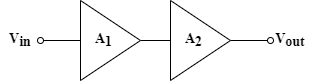
\includegraphics[width=0.4\linewidth]{cascaded}
		\caption{An example of a cascaded amplifier.}
		\label{fig:cascaded}
	\end{figure}
	
	Since the phase shift must be minimized, we can either use two inverting amplifiers or simply use non-inverting amplifiers. Additionally, as the input resistance is required to be high ($\ge \SI{1}{\Mohm}$) it seems that a non-inverting amplifier would be the best option, as an ideal non-inverting amplifier configuration has an infinite resistance. There are several combinations of two or three non-inverting amplifiers that can be used to achieve the \SI{1000}{\V/\V} goal. A few options are considered are: \begin{align*}
		G_1 & = 10 \times 100 \\
		G_2 & = 10 \times 10 \times 10 \\
		G_3 & = 20 \times 50 \\
		G_4 & = 25 \times 40
	\end{align*}
	The third option, $A_1 = 20$ and $A_2 = 50$, was chosen as it was used as the example in-class and had a straight-forward calculation. To achieve this, we can use the gain for a non-ideal non-inverting op amps and approximate the gain to
	\begin{subequations}
		\begin{align}
			G \equiv \frac{V_\mathrm{out}}{V_\mathrm{in}} & = \frac{1 + R_2 / R_1}{1 + \frac{1 + (R_2 / R_1)}{A}} \\
			G & \approx \frac{1 + R_2 / R_1}{1 + \frac{R_2 / R_1}{A}} \label{eq:exp2gain}
		\end{align}
	\end{subequations}

	In OrCAD, a circuit was built with two non-inverting op amps and simulated using PSPICE, showing an ideal gain of \SI{1000}{\V/\V}. This circuit is shown in Figure \ref{fig:exp2orcad}. To accomplish this, four resistors were used: on the first amplifier with gain \SI{20}{\V/\V}, $R_1=\SI{1}{\kohm}$ and $R_2=\SI{20}{\kohm}$. On the second amplifier, $R_3=\SI{1}{\kohm}$ and $R_4=\SI{50}{\kohm}$, leading to gain of \SI{50}{\V/\V}.
	
	\begin{figure}[h]
		\centering
		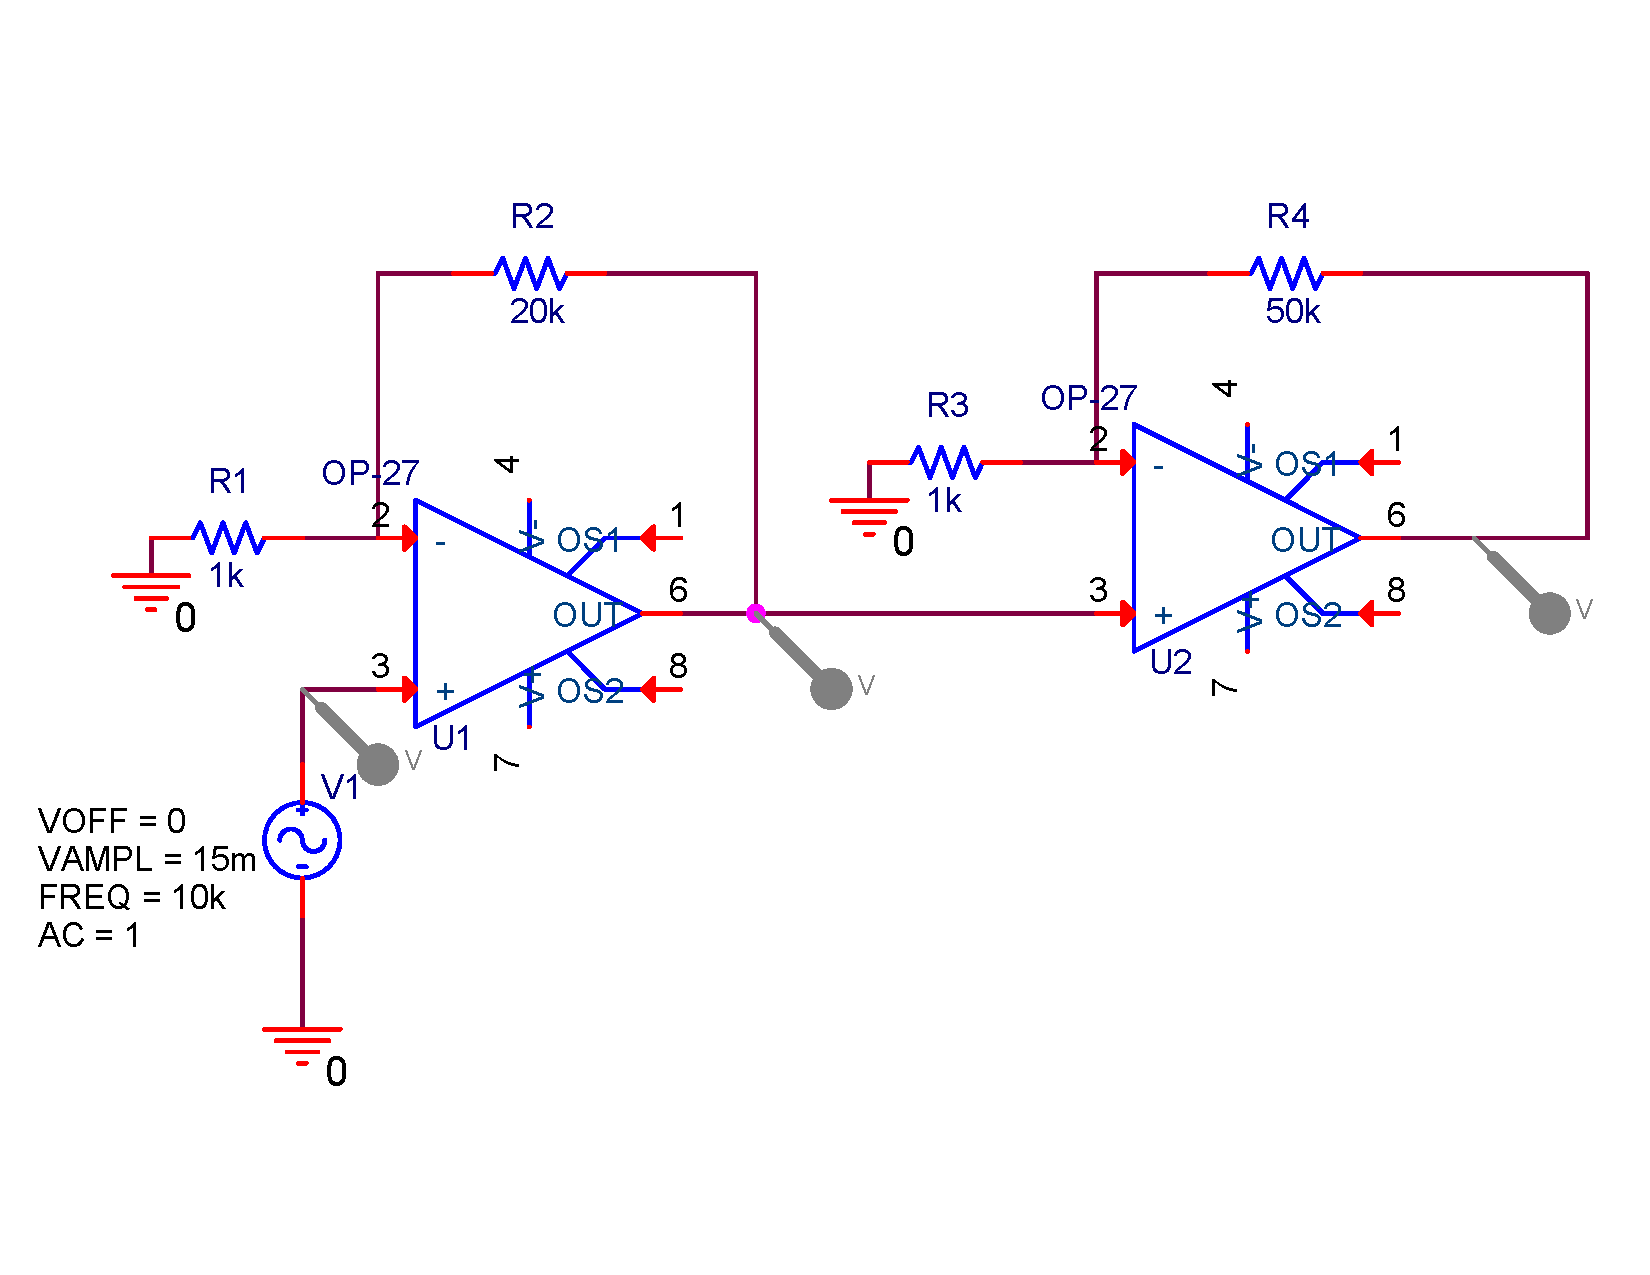
\includegraphics[width=0.7\linewidth, trim=0 80 0 80, clip]{exp2orcad}
		\caption{The cascading amplifiers used in Experiment 2.}
		\label{fig:exp2orcad}
	\end{figure}
	
	
	\subsection{Procedure}
	The follow steps were carried out, as instructed by the lab assignment.
	
	\begin{enumerate}
		\item The 2-stage amplifier circuit was designed, noted in the theoretical background section above. 
		\item The expected gains were calculated using \eqref{eq:exp2gain}, for both the individual amplifier stages and the product of both stages. This was simulated in PSPICE.
		\item The circuit was implemented on the breadboard and each amplifier stage was tested individually before they were combined.
		\item The gain was tested and recorded using various input voltages within the range of the requirements.
		\item The input resistance was measured using a \SI{1}{\Mohm} sense resistor across the input. This was done by attaching a 10X probe across the resistor and calculating the current through it. \label{step:last}
		\item The output resistance was measured by using a \SI{470}{\ohm} resistor and later, a \SI{10}{\kohm} resistor on the output of the second op amp. This was done by using a similar technique to Step \ref{step:last}.
	\end{enumerate}

	\pagebreak
	\subsection{Results and analysis}
	% state all measured values, graphs, tables, and figs.
	% state any deviation from theoretical expected values
	% use tables and graphs
	% * must justify error in results otherwise the experiment failed
	
	\subsubsection{Measured component values}
	The components of Figure \ref{fig:exp2orcad} were measured and recorded in Table \ref{table:lab2components}.
	
	\begin{table}[H]
		\centering
		\caption{Experimental and nominal component values.}
		\label{table:lab2components}
		\begin{threeparttable}
			\begin{tabular}{cccc}
				\toprule
				Component & Nominal & Measured & \% Error (Tolerance) \\
				\midrule
				$R_1$ & \SI{1}{\kohm} & \SI{0.9724}{\kohm} & 2.76\% (5\%) \\
				$R_2$ & \SI{20}{\kohm} & \SI{19.454}{\kohm} & 2.73\% (5\%) \\
				$R_3$ & \SI{1}{\kohm} & \SI{1.0198}{\kohm} & 1.98\% (5\%) \\
				$R_4$ & \SI{50}{\kohm} & \SI{48.79}{\kohm} & 2.42\% (5\%) \\
				\midrule
				$R_\mathrm{test-in}$ & \SI{1}{\Mohm} & \SI{0.9827}{\Mohm} & 1.73\% (5\%) \\
				$R_\mathrm{test-out1}$ & \SI{470}{\ohm} & \SI{463.3}{\ohm} & 1.42\% (5\%) \\
				$R_\mathrm{test-out2}$ & \SI{10}{\kohm} & \SI{9.719}{\kohm} & 2.81\% (5\%) \\
				\bottomrule
			\end{tabular}
		\end{threeparttable}
	\end{table}
	
	\subsubsection{Amplifier stages and total gain}
	The gain of the individual amplifiers were tested separately before cascading. This was accomplished using an input $V_\mathrm{in} = \SI{1}{\milli\Vpp}$ at \SI{10}{\kHz}. Despite some error during the individual amplifier testing, when combined, there was an exact \SI{1000.0}{\V/\V} gain across the entire amplifier, as shown in Figure \ref{fig:f0005tek}. This could be due to additional impedances in the connecting wire or the breadboard. The values and error of the stages are noted in Table \ref{table:lab2gainvalues} below.
	
	\begin{table}[H]
		\centering
		\caption{Ideal (nominal), predicted, and measured gain. The predicted gains are calculated using \eqref{eq:exp2gain} and the actual resistor values from Table \ref{table:lab2components}.}
		\label{table:lab2gainvalues}
		\begin{threeparttable}
			\begin{tabular}{ccccc}
				\toprule
				Stage & Ideal & Predicted & Measured & Error \\
				\midrule
				$A_1$ & \SI{20}{\V/\V} & \SI{20.77}{\V/\V} & \SI{20.4}{\V/\V} & $+2.0\%$ \\
				$A_2$ & \SI{50}{\V/\V} & \SI{47.56}{\V/\V} & \SI{49.6}{\V/\V} & $-0.8\%$ \\
				$A_1 A_2$ & \SI{1000}{\V/\V} & \SI{1011.84}{\V/\V} & \SI{1000.0}{\V/\V} & $0\%$ \\
				\bottomrule
			\end{tabular}
		\end{threeparttable}
	\end{table}

	\begin{figure}[h]
		\centering
		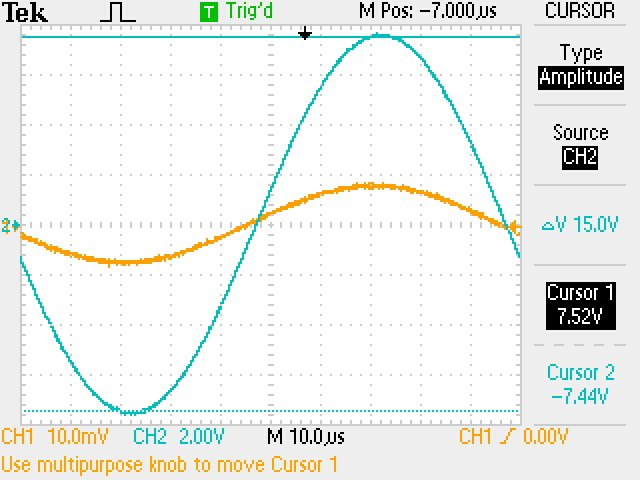
\includegraphics[width=0.5\linewidth]{scope/F0005TEK}
		\caption{The measurement of the output gain showing an ideal \SI{1000}{\V/\V} gain and minimal phase shift.}
		\label{fig:f0005tek}
	\end{figure}
	
	\subsubsection{Input and output resistances}
	The voltage across the amplifier was found to be \SI{11.2}{\mV}. Using a voltage divider, with $R_\mathrm{test-in}$ in series with the input amplifier, the input resistance can be calculated as, \begin{align}
		V_\mathrm{div} & = \frac{ R_\mathrm{in} }{R_\mathrm{test-in} + R_\mathrm{in}} V_\mathrm{in} \notag \\
		R_\mathrm{in} & = \frac{R_\mathrm{test-in}}{V_\mathrm{in} / V_\mathrm{div} - 1} = \frac{\SI{0.9827}{\Mohm}}{20.0 / 11.2 - 1} \notag \\
			& = \SI{1.25}{\Mohm} \notag
	\end{align}
	
	Using the \SI{470}{\ohm} resistor, the output voltage dropped significantly from the open-circuit voltage $V_\mathrm{OC}= \SI{10.0}{\V}$ to \SI{9.36}{\V}. This is likely because the op amp was unable to supply the needed current ($\approx \SI{20}{\mA}$). This is evident by viewing Figure 24 in the OP27 datasheet (excerpt provided in the Appendix). This figure shows at loads under $\SI{1}{\kohm}$, the op amp is unable to supply the maximum output voltage of $\pm V_s$. Only once it exceeds a load of $\SI{1}{\kohm}$ does the maximum output voltage (and current) become linear and under this load resistance value, the region is non-linear and drops substantially. This demonstrates the need for a higher load resistance.
	
	As recommended during the lecture, this resistor was switched out for a \SI{10}{\kohm}. Using the standard voltage divider, we can determine the output resistance $R_\mathrm{out}$ as \begin{align*}
		R_\mathrm{out} & = R_\mathrm{test-out} \left(\frac{V_\mathrm{OC}}{V_\mathrm{out} - 1}\right) \\
			& = \left(\SI{9.719}{\kohm}\right) \left( \frac{10.0}{9.92} - 1 \right) \\
			& = \SI{78.4}{\ohm}
	\end{align*}
	This output resistance does not meet the required specifications of this project. This is likely additionally due to the internal impedances of the probe, as well as the non-ideal characteristics of the breadboard and OP27 op amps.
	
	\subsection{Conclusion}
	%  conclusion of the exp
	This experiment demonstrated using cascading op amps in a design to exceed the open-loop gain of a single op amp. The OP27 op amp has several limitations that must be accounted for, especially in a design with strict requirements. The low output resistance requirement in this experiment was not met, likely due to the additional impedances of the setup and non-ideal characteristics of the breadboard and probes.
	
%	\printbibliography
	 
	\pagebreak
	
	\section*{Appendix}
	\begin{figure}[h]
		\centering
		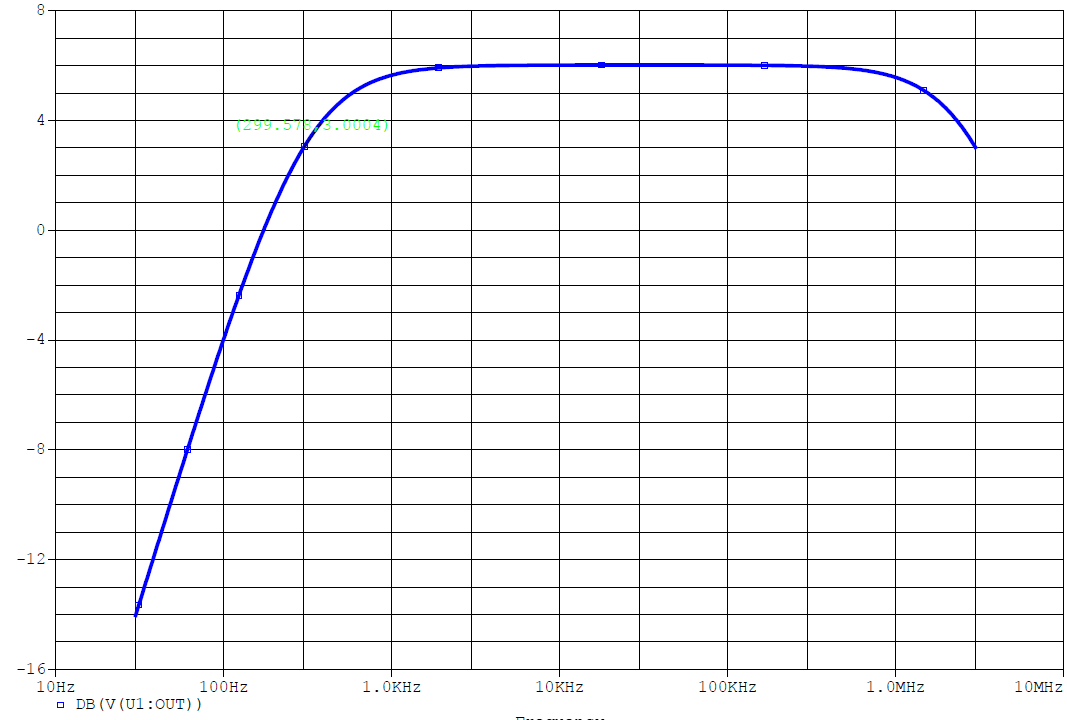
\includegraphics[width=\linewidth]{exp1simscreenshot}
		\caption{Bode plot of the frequency response of the simulated circuit in Experiment 1.}
		\label{fig:exp1simscreenshot}
	\end{figure}

	\begin{figure}[h]
		\centering
		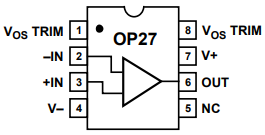
\includegraphics[width=0.4\linewidth]{exp1pinout}
		\caption{Pinout of the Analog OP27 op amp.}
		\label{fig:exp1pinout}
	\end{figure}

\begin{figure}
	\centering
	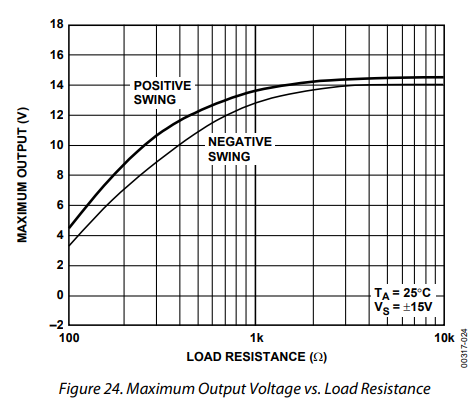
\includegraphics[width=0.7\linewidth]{op27fig24}
	\caption{Excerpt of the OP27 datasheet.}
	\label{fig:op27fig24}
\end{figure}

\end{document}